\section{Data description, visualization and statistical analysis} \label{data-visualization}

We used a dataset given by the teacher containing two distinct folders: one with face image examples and the other with non-face image examples. The images are in gray scale and weren't normalized as can be seen in figures \ref{fig:faces-overview} and \ref{fig:non-faces-overview}.

\begin{figure}[htbp]
\centerline{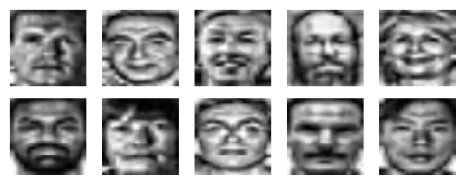
\includegraphics[scale=0.35]{images/faces_overview.png}}
\caption{Overview of the images with faces in the dataset.}
\label{fig:faces-overview}
\end{figure}

\begin{figure}[htbp]
\centerline{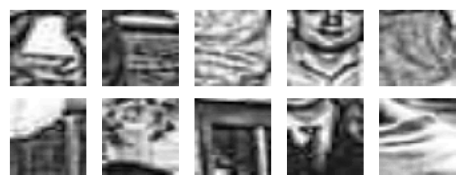
\includegraphics[scale=0.35]{images/non_faces_overview.png}}
\caption{Overview of the images without faces in the dataset.}
\label{fig:non-faces-overview}
\end{figure}

This dataset contains 124 images, 69 of which are face images and 55 are non-face images, with a window of pixels of \(27 \times 18\). We can conclude that the dataset is a little skewed, having more face images than non-face images as it is represented in figure \ref{fig:dataset-distribution}.

\begin{figure}[htbp]
\centerline{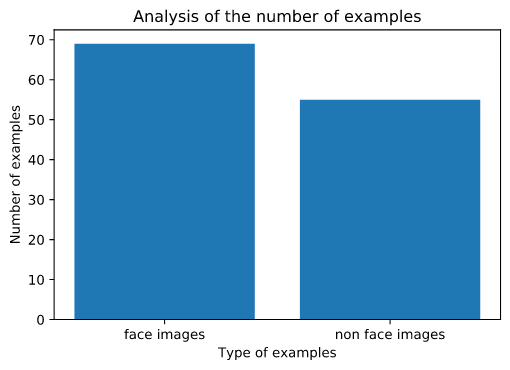
\includegraphics[scale=0.35]{images/data_distribution.png}}
\caption{Analysis of the number of examples for each type of image.}
\label{fig:dataset-distribution}
\end{figure}